\subsubsection{OpenCV 简介与环境}

OpenCV（Open Source Computer Vision Library）是视觉组最常用的 C++ 图像处理库，
提供矩阵式图像表示、色彩空间转换、滤波、形态学、轮廓与特征等能力。
卷一 CMake 章已介绍 \texttt{find\_package(OpenCV REQUIRED)}，本节补齐安装与链接细节。

构建命令用于生成并执行编译规则，通用形式为 $cmake\enspace [OPTIONS]$。
\begin{center}
\begin{tabular}{lp{0.6\textwidth}}
\toprule[1.5pt]
参数 & 作用 \\
\midrule[1pt]
\texttt{-S PATH} & 指定源码目录 \\
\texttt{-B PATH} & 指定构建目录 \\
\texttt{--build PATH} & 构建已配置的目录 \\
\texttt{--target NAME} & 构建指定目标，与 --build 配合 \\
\texttt{-DNAME=VALUE} & 设置 CMake 缓存变量 \\
\bottomrule[1.5pt]
\end{tabular}
\end{center}
其余参数请查阅 cmake 帮助或 man 手册。

Ubuntu 22.04 上可通过 apt 安装开发包：
\begin{tbash}
sudo apt update
sudo apt install libopencv-dev
pkg-config --modversion opencv4
\end{tbash}

CMake 中推荐写法（OpenCV 4.x）：
\begin{tcode}
cmake_minimum_required(VERSION 3.16)
project(image_demo LANGUAGES CXX)
find_package(OpenCV REQUIRED)
message(STATUS "OpenCV: ${OpenCV_VERSION}")
add_executable(demo main.cpp)
target_include_directories(demo PRIVATE ${OpenCV_INCLUDE_DIRS})
target_link_libraries(demo PRIVATE ${OpenCV_LIBS})
\end{tcode}

常用头文件：\texttt{opencv2/opencv.hpp} 可一次引入核心模块；


仅处理图像时也可分别包含 \texttt{opencv2/core.hpp}、\texttt{imgproc.hpp}、\texttt{highgui.hpp}、\texttt{imgcodecs.hpp}、\texttt{videoio.hpp}。

\begin{example}
把本章任一完整 C++ 示例保存为 main.cpp，将上面的配置保存为 CMakeLists.txt。
先用下列程序确认链接成功：
\begin{tcode}
#include <opencv2/opencv.hpp>
#include <iostream>
#include <vector>
int main() {
    std::cout << CV_VERSION << "\n";
}
\end{tcode}
\end{example}

\begin{example}
构建命令通用形式为 $cmake\enspace [OPTIONS]$；-S 指定源码目录，-B 指定构建目录，--build 执行构建。其余选项查阅 cmake 帮助或 man 手册。本章固定使用独立构建目录。
\begin{tbash}
cmake -S . -B build
cmake --build build
./build/demo
\end{tbash}
\end{example}

\begin{exercise}
将目标名 demo 改为 image\_demo，重新配置、构建并运行。写出源码目录与构建目录分别在哪里。
\end{exercise}

\subsubsection{Mat：图像的核心数据结构}

\texttt{cv::Mat} 是 OpenCV 的核心类型，表示二维（或多维）数组。
彩色图通常为三通道 8 位无符号整数，类型记为 \texttt{CV\_8UC3}；灰度图为 \texttt{CV\_8UC1}。

\begin{itemize}
    \item \textbf{尺寸：}\texttt{rows}、\texttt{cols}、\texttt{channels()}、\texttt{size()}
    \item \textbf{类型：}\texttt{type()}、\texttt{depth()}（如 \texttt{CV\_8U}）
    \item \textbf{判空：}\texttt{empty()}，读图失败时必须检查
\end{itemize}

\textbf{浅拷贝与深拷贝。}
赋值与拷贝构造只复制表头，底层数据共享；修改一方会影响另一方。
需要独立副本时使用 \texttt{clone()} 或 \texttt{copyTo()}：
\begin{tcode}
cv::Mat A = cv::imread("input.jpg");
cv::Mat B = A;          // 共享数据
cv::Mat C = A.clone();  // 深拷贝
\end{tcode}

\textbf{像素访问。}BGR 三通道常用 \texttt{at}：
\begin{tcode}
cv::Vec3b px = img.at<cv::Vec3b>(y, x); // 注意顺序：行 y，列 x
uchar b = px[0], g = px[1], r = px[2];  // OpenCV 默认 BGR
\end{tcode}
性能敏感路径可用指针逐行扫描（\texttt{ptr<T>(row)}），避免对每个像素调用 \texttt{at}。

\textbf{ROI（Region of Interest，感兴趣区域）。}以下调用与原图共享内存：
\begin{tcode}
cv::Mat roi = img(cv::Rect(x, y, w, h));
\end{tcode}
若需独立处理，对 ROI 再 \texttt{clone()}。

\begin{example}
验证共享数据与独立副本。输出应为 9 1。
\begin{tcode}
#include <opencv2/opencv.hpp>
#include <iostream>
#include <vector>
int main() {
    cv::Mat a(2, 2, CV_8UC1, cv::Scalar(1));
    cv::Mat b = a, c = a.clone();
    b.at<uchar>(0, 0) = 9;
    std::cout << int(a.at<uchar>(0, 0)) << " "
              << int(c.at<uchar>(0, 0)) << "\n";
}
\end{tcode}
\end{example}

\begin{exercise}
将 b 改为 a 的单像素 ROI，重复修改。解释为什么 ROI 与 clone 的结果不同。
\end{exercise}

\begin{conclusion}
\begin{itemize}
\item Mat 表头保存尺寸和类型，数据可能被多个表头共享。
\item ROI 仍共享原图，clone 创建独立数据。
\item 访问像素先核对行列、通道和类型，再考虑性能。
\end{itemize}
\end{conclusion}

\subsubsection{图像与视频的读写}

\paragraph*{文件读写与窗口显示}
\begin{tcode}
#include <opencv2/opencv.hpp>
int main() {
    cv::Mat img = cv::imread("input.jpg", cv::IMREAD_COLOR);
    if (img.empty()) return -1;
    cv::namedWindow("demo", cv::WINDOW_AUTOSIZE);
    cv::imshow("demo", img);
    int key = cv::waitKey(0); // 0 表示一直等待按键
    if (key == 's') cv::imwrite("output.png", img);
    return 0;
}
\end{tcode}

\texttt{imread} 常用标志：\texttt{IMREAD\_COLOR}（默认 BGR 三通道）、
\texttt{IMREAD\_GRAYSCALE}、\texttt{IMREAD\_UNCHANGED}（保留 alpha 等）。
\texttt{imwrite} 根据扩展名选择编码格式。

\paragraph*{摄像头与视频流}
\begin{example}
设备就绪后运行以下完整程序，按 Esc 退出。保存为 main.cpp，使用本章首节构建配置。
\begin{tcode}
#include <opencv2/opencv.hpp>
int main() {
cv::VideoCapture cap(0); // 0 为默认摄像头；也可填视频路径
if (!cap.isOpened()) return -1;
cv::Mat frame;
while (true) {
    if (!cap.read(frame) || frame.empty()) break;
    cv::imshow("cam", frame);
    if (cv::waitKey(1) == 27) break; // Esc 退出
}
    return 0;
}
\end{tcode}
\end{example}

可用 \texttt{cap.set(cv::CAP\_PROP\_FRAME\_WIDTH, 1280)} 等属性尝试设定分辨率；
实际是否生效取决于驱动与设备。

\begin{example}
生成本地图像再读取，无摄像头也能检查文件路径。应输出 32 48。
\begin{tcode}
#include <opencv2/opencv.hpp>
#include <iostream>
#include <vector>
int main() {
    cv::Mat a(32, 48, CV_8UC3, cv::Scalar(0, 255, 0));
    if (!cv::imwrite("input.png", a)) return 1;
    cv::Mat b = cv::imread("input.png");
    if (b.empty()) return 2;
    std::cout << b.rows << " " << b.cols << "\n";
}
\end{tcode}
\end{example}

\begin{exercise}
把读取路径改为不存在的文件，确认程序返回 2；说明为何读图后必须先判空。
\end{exercise}

\subsubsection{色彩空间与颜色分割}

OpenCV 默认彩色图为 \textbf{BGR}，不是 RGB。灰度转换：
\begin{tcode}
cv::Mat gray;
cv::cvtColor(img, gray, cv::COLOR_BGR2GRAY);
\end{tcode}

识别任务中常转到 \textbf{HSV}：H 表示色调，S 饱和度，V 亮度。
在 8 位图上，OpenCV 的范围为 $H\in[0,179]$，$S,V\in[0,255]$
（与部分图像软件的 $H\in[0,360]$ 不同，换算时需注意）。

颜色分割用 \texttt{inRange} 生成二值掩膜，再用按位与提取前景：
\begin{tcode}
cv::Mat hsv, mask, result;
cv::cvtColor(img, hsv, cv::COLOR_BGR2HSV);
cv::inRange(hsv, cv::Scalar(100, 50, 50), cv::Scalar(130, 255, 255), mask); // 蓝示例
cv::bitwise_and(img, img, result, mask);
\end{tcode}

\textbf{红色的特殊处理。}红色落在色环两端附近，需两段区间再合并：
\begin{tcode}
cv::Mat m1, m2, mask;
cv::inRange(hsv, cv::Scalar(0, 70, 50), cv::Scalar(10, 255, 255), m1);
cv::inRange(hsv, cv::Scalar(170, 70, 50), cv::Scalar(179, 255, 255), m2);
mask = m1 | m2;
\end{tcode}
阈值需按光照与相机标定；可用取色工具或把单像素 BGR 转 HSV 后估计中心色相。

\begin{example}
直接构造色环两端的两个红色像素和一个蓝色像素，掩膜非零数应为 2。
\begin{tcode}
#include <opencv2/opencv.hpp>
#include <iostream>
#include <vector>
int main() {
    cv::Mat hsv(1, 3, CV_8UC3);
    hsv.at<cv::Vec3b>(0, 0) = {0, 255, 255};
    hsv.at<cv::Vec3b>(0, 1) = {179, 255, 255};
    hsv.at<cv::Vec3b>(0, 2) = {120, 255, 255};
    cv::Mat a, b, mask;
    cv::inRange(hsv, cv::Scalar(0,70,50), cv::Scalar(10,255,255), a);
    cv::inRange(hsv, cv::Scalar(170,70,50), cv::Scalar(179,255,255), b);
    cv::bitwise_or(a, b, mask);
    std::cout << cv::countNonZero(mask) << "\n";
}
\end{tcode}
\end{example}

\begin{exercise}
把第二个像素色调改为 90，预测并验证结果；再把第一个像素饱和度设为 0。
\end{exercise}

\subsubsection{阈值分割}

滤波与轮廓之前，常把灰度图转为二值图。

\textbf{固定阈值：}
\begin{tcode}
cv::Mat binary;
cv::threshold(gray, binary, 127, 255, cv::THRESH_BINARY);
\end{tcode}

\textbf{Otsu 自动阈值}（适合双峰直方图）：
\begin{tcode}
cv::threshold(gray, binary, 0, 255, cv::THRESH_BINARY | cv::THRESH_OTSU);
\end{tcode}

\textbf{自适应阈值}（光照不均时更稳）：
\begin{tcode}
cv::adaptiveThreshold(gray, binary, 255,
    cv::ADAPTIVE_THRESH_GAUSSIAN_C, cv::THRESH_BINARY, 11, 2);
\end{tcode}
其中块大小须为奇数；常数项用于微调局部阈值。

\begin{example}
用三像素灰度图检查固定阈值的边界，结果应为 0 0 255。
\begin{tcode}
#include <opencv2/opencv.hpp>
#include <iostream>
#include <vector>
int main() {
    cv::Mat gray = (cv::Mat_<uchar>(1,3) << 126,127,128);
    cv::Mat binary;
    cv::threshold(gray, binary, 127, 255, cv::THRESH_BINARY);
    for (int x=0; x<3; ++x) std::cout << int(binary.at<uchar>(0,x)) << " ";
    std::cout << "\n";
}
\end{tcode}
\end{example}

\begin{exercise}
改用 THRESH\_BINARY\_INV，先预测输出，再运行验证。
\end{exercise}

\subsubsection{滤波与降噪}

相机图像常含噪声。常见类型包括高斯噪声、椒盐噪声等。

\begin{figure}[H]
    \centering
    \begin{subfigure}{0.48\textwidth}
        \centering
        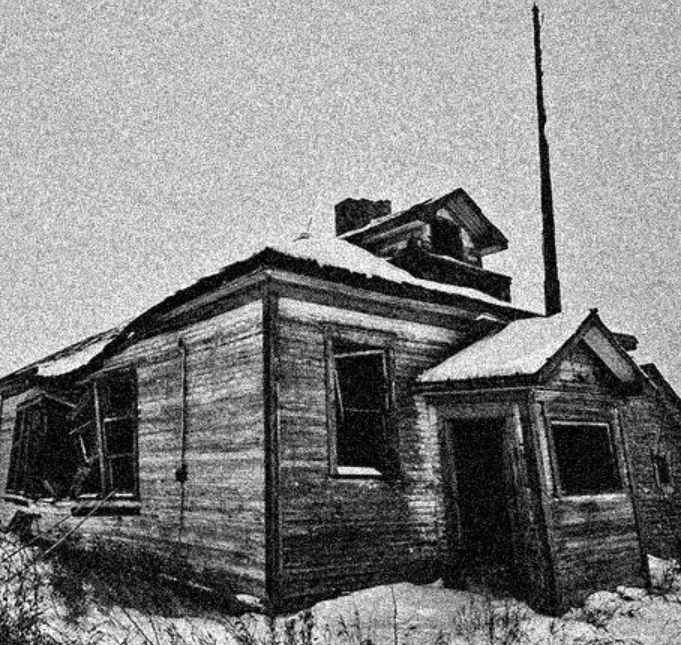
\includegraphics[width=\linewidth]{gaussian.png}
        \caption{高斯噪声}
    \end{subfigure}
    \hfill
    \begin{subfigure}{0.48\textwidth}
        \centering
        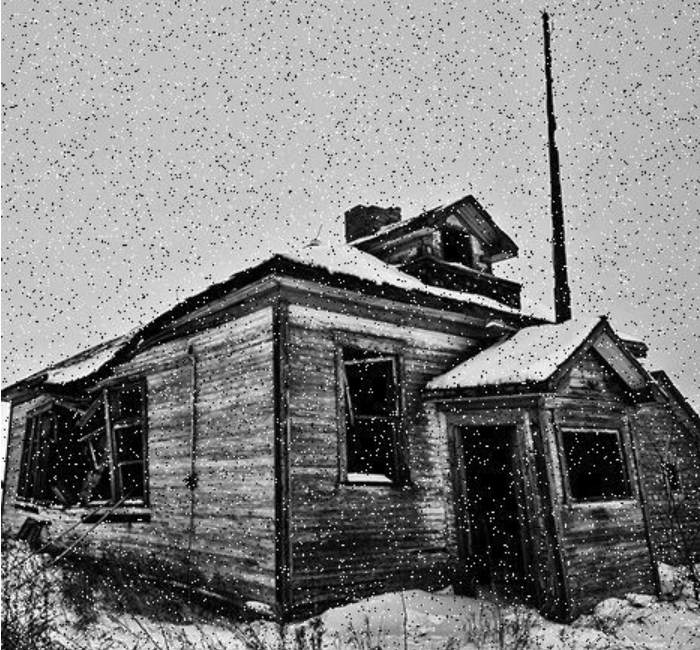
\includegraphics[width=\linewidth]{salt.png}
        \caption{椒盐噪声}
    \end{subfigure}
    \caption{常见图像噪声示例}
\label{fig:B_opencv-1}
\end{figure}

\begin{itemize}
    \item \texttt{cv::blur}：均值滤波，速度快，边缘易糊。
    \item \texttt{cv::GaussianBlur}：高斯加权，核宽高须为奇数；\texttt{$\sigma$} 可设为 $0$ 由核大小推断。
    \item \texttt{cv::medianBlur}：中值滤波，对椒盐噪声更有效。
    \item \texttt{cv::bilateralFilter}：双边滤波，平滑时尽量保边，计算更重。
\end{itemize}

\begin{tcode}
cv::Mat blurred;
cv::GaussianBlur(img, blurred, cv::Size(5, 5), 0);
cv::medianBlur(img, blurred, 5); // ksize 为奇数
\end{tcode}

边缘检测前通常先做轻度高斯模糊，以抑制噪声引起的伪边缘。

\begin{example}
用中值滤波去除孤立亮点，中心像素应从 255 变成 0。
\begin{tcode}
#include <opencv2/opencv.hpp>
#include <iostream>
#include <vector>
int main() {
    cv::Mat a = cv::Mat::zeros(7, 7, CV_8UC1), out;
    a.at<uchar>(3,3) = 255;
    cv::medianBlur(a, out, 3);
    std::cout << int(out.at<uchar>(3,3)) << "\n";
}
\end{tcode}
\end{example}

\begin{exercise}
改用 3×3 均值滤波，比较中心值；解释均值和中值为何不同。
\end{exercise}

\subsubsection{形态学操作}

形态学在二值图上用结构元素（核）做邻域运算，可去噪、填孔、连接断裂区域。

\begin{itemize}
    \item \textbf{腐蚀 \texttt{erode}}：缩小前景，去除毛刺。
    \item \textbf{膨胀 \texttt{dilate}}：扩大前景，弥合缝隙。
    \item \textbf{开运算}：先腐蚀后膨胀，去小噪点。
    \item \textbf{闭运算}：先膨胀后腐蚀，填小孔洞。
\end{itemize}

\begin{tcode}
cv::Mat kernel = cv::getStructuringElement(cv::MORPH_RECT, cv::Size(3, 3));
cv::Mat opened, closed;
cv::morphologyEx(binary, opened, cv::MORPH_OPEN, kernel);
cv::morphologyEx(binary, closed, cv::MORPH_CLOSE, kernel);
\end{tcode}

核形状可选 \texttt{MORPH\_RECT}、\texttt{MORPH\_ELLIPSE}、\texttt{MORPH\_CROSS}；
核越大，效果越强，也越容易抹掉细节。灯条等细长结构有时用椭圆核更合适。

\begin{example}
开运算去除孤立点，保留 5×5 方块。非零数应从 26 变成 25。
\begin{tcode}
#include <opencv2/opencv.hpp>
#include <iostream>
#include <vector>
int main() {
    cv::Mat a = cv::Mat::zeros(12,12,CV_8UC1), out;
    a(cv::Rect(4,4,5,5)).setTo(255);
    a.at<uchar>(1,1)=255;
    auto k=cv::getStructuringElement(cv::MORPH_RECT,cv::Size(3,3));
    cv::morphologyEx(a,out,cv::MORPH_OPEN,k);
    std::cout << cv::countNonZero(a) << " " << cv::countNonZero(out) << "\n";
}
\end{tcode}
\end{example}

\begin{exercise}
将核改为 7×7，检查方块能否保留。说明“大核去噪更强”的代价。
\end{exercise}

\begin{conclusion}
\begin{itemize}
\item 腐蚀缩前景，膨胀扩前景。
\item 开运算先腐蚀，闭运算先膨胀，二者顺序不可交换。
\item 核尺寸要与目标宽度比较；先保存中间图，再继续调参。
\end{itemize}
\end{conclusion}

\subsubsection{边缘检测与轮廓}

\paragraph*{Canny}
Canny 流程：高斯平滑 $\rightarrow$ 梯度 $\rightarrow$ 非极大值抑制 $\rightarrow$ 双阈值滞后。
两个阈值常用约 $1:2$ 或 $1:3$ 的比例：
\begin{tcode}
cv::Mat edges;
cv::Canny(gray, edges, 50, 150);
\end{tcode}

\paragraph*{轮廓提取与几何筛选}
\begin{tcode}
std::vector<std::vector<cv::Point>> contours;
std::vector<cv::Vec4i> hierarchy;
cv::findContours(edges, contours, hierarchy,
                 cv::RETR_EXTERNAL, cv::CHAIN_APPROX_SIMPLE);

for (const auto& c : contours) {
    double area = cv::contourArea(c);
    if (area < 100.0) continue; // 面积阈值按场景调整
    cv::RotatedRect rr = cv::minAreaRect(c);
    cv::Point2f pts[4];
    rr.points(pts);
    for (int i = 0; i < 4; ++i)
        cv::line(img, pts[i], pts[(i + 1) % 4], cv::Scalar(0, 255, 0), 2);
}
\end{tcode}

\begin{itemize}
    \item \texttt{RETR\_EXTERNAL}：只取最外层轮廓；\texttt{RETR\_TREE} 保留层级。
    \item \texttt{CHAIN\_APPROX\_SIMPLE}：压缩共线点，节省存储。
    \item 常用几何量：\texttt{contourArea}、\texttt{arcLength}、\texttt{boundingRect}、
          \texttt{minAreaRect}、\texttt{approxPolyDP}。
\end{itemize}

赛场上灯条、装甲板的具体面积比、长宽比与角度阈值见卷三；本卷先掌握工具。

\begin{example}
从实心矩形提取轮廓。应有 1 条外轮廓；连续几何面积为 171，非零像素为 200。
\begin{tcode}
#include <opencv2/opencv.hpp>
#include <iostream>
#include <vector>
int main() {
    cv::Mat a=cv::Mat::zeros(40,40,CV_8UC1);
    a(cv::Rect(5,5,20,10)).setTo(255);
    std::vector<std::vector<cv::Point>> cs;
    cv::findContours(a,cs,cv::RETR_EXTERNAL,cv::CHAIN_APPROX_SIMPLE);
    if(cs.size()!=1) return 1;
    std::cout << cs.size() << " " << cv::contourArea(cs[0]) << " "
              << cv::countNonZero(a) << "\n";
}
\end{tcode}
\end{example}

\begin{exercise}
对同一图运行 Canny 再提轮廓，比较数量与面积。说明像素数为何不总等于 contourArea。
\end{exercise}

\subsubsection{几何变换与绘图}

\textbf{缩放：}
\begin{tcode}
cv::Mat small;
cv::resize(img, small, cv::Size(), 0.5, 0.5, cv::INTER_AREA); // 缩小常用 AREA
\end{tcode}
放大可选用 \texttt{INTER\_LINEAR} 或 \texttt{INTER\_CUBIC}。

\textbf{旋转（绕中心）：}
\begin{tcode}
cv::Point2f center(img.cols / 2.0f, img.rows / 2.0f);
cv::Mat rotated;
cv::Mat M = cv::getRotationMatrix2D(center, 30.0, 1.0); // 角度、缩放
cv::warpAffine(img, rotated, M, img.size());
\end{tcode}

\textbf{常用绘图：}\texttt{line}、\texttt{rectangle}、\texttt{circle}、\texttt{putText}。
颜色仍按 BGR，例如绿色为 \texttt{Scalar(0,255,0)}。

\begin{example}
把 80×40 图像缩为一半，应得到 40×20；输出文件名为 small.png。
\begin{tcode}
#include <opencv2/opencv.hpp>
#include <iostream>
#include <vector>
int main() {
    cv::Mat a(40,80,CV_8UC3,cv::Scalar(0,0,0)), small;
    cv::circle(a,cv::Point(40,20),10,cv::Scalar(0,255,0),-1);
    cv::resize(a,small,cv::Size(),0.5,0.5,cv::INTER_AREA);
    if(!cv::imwrite("small.png",small)) return 1;
    std::cout << small.cols << " " << small.rows << "\n";
}
\end{tcode}
\end{example}

\begin{exercise}
按最近邻方式缩放，与 INTER\_AREA 比较圆边缘；说明插值选择与图像用途的关系。
\end{exercise}

\subsubsection{传统特征与匹配入门}

深度学习普及前，SIFT、ORB 等手工特征用于定位与匹配。
OpenCV 提供 \texttt{cv::ORB::create()}、\texttt{detectAndCompute} 与
\texttt{cv::BFMatcher} / \texttt{FlannBasedMatcher}。
视觉组日常识别以神经网络为主；在纹理稳定、算力受限或需要快速原型时，
ORB 仍可作为补充。深入匹配与位姿估计可结合相机标定与几何视觉章节。

\begin{example}
匹配相同图像的 ORB 描述子，匹配距离应全部为零；特征数量依版本略有差异。
\begin{tcode}
#include <opencv2/opencv.hpp>
#include <iostream>
#include <vector>
int main() {
    cv::Mat a(240,320,CV_8UC1);
    cv::RNG rng(42); rng.fill(a,cv::RNG::UNIFORM,0,256);
    auto orb=cv::ORB::create();
    std::vector<cv::KeyPoint> kp; cv::Mat desc;
    orb->detectAndCompute(a,cv::noArray(),kp,desc);
    if(desc.empty()) return 1;
    std::vector<cv::DMatch> matches;
    cv::BFMatcher(cv::NORM_HAMMING,true).match(desc,desc,matches);
    for(const auto& m:matches) if(m.distance!=0) return 2;
    std::cout << matches.size() << "\n";
}
\end{tcode}
\end{example}

\begin{exercise}
将图像平移 5 像素再匹配，记录匹配数量。说明低距离为何不能单独证明几何关系正确。
\end{exercise}

\subsubsection{与 ROS2 集成：cv\_bridge}

ROS2 中相机话题类型为 \texttt{sensor\_msgs/msg/Image}，
经 \texttt{cv\_bridge} 与 \texttt{cv::Mat} 互转。转换可能抛出异常，应捕获：
\begin{tcode}
#include <cv_bridge/cv_bridge.h>
#include <sensor_msgs/image_encodings.hpp>

void callback(const sensor_msgs::msg::Image::ConstSharedPtr& msg) {
    cv_bridge::CvImagePtr cv_ptr;
    try {
        cv_ptr = cv_bridge::toCvCopy(msg, sensor_msgs::image_encodings::BGR8);
    } catch (const cv_bridge::Exception& e) {
        RCLCPP_ERROR(rclcpp::get_logger("demo"), "cv_bridge: %s", e.what());
        return;
    }
    cv::Mat frame = cv_ptr->image;
    // ... OpenCV 处理 ...
    sensor_msgs::msg::Image out_msg;
    cv_bridge::CvImage(msg->header, sensor_msgs::image_encodings::BGR8, frame)
        .toImageMsg(out_msg);
    publisher_->publish(out_msg);
}
\end{tcode}

功能包须在 \texttt{package.xml} 与 \texttt{CMakeLists.txt} 中声明
\texttt{cv\_bridge}、\texttt{sensor\_msgs} 依赖。可与第一章工作空间练习合并验收。

\begin{example}
无需相机的往返转换。保存为 bridge.cpp，在已加载 Humble 环境的 ament 包中声明 rclcpp、cv\_bridge、sensor\_msgs、std\_msgs 依赖，并用下方配置构建。输出应为 8 8。
\begin{tcode}
#include <cv_bridge/cv_bridge.h>
#include <sensor_msgs/image_encodings.hpp>
#include <iostream>
int main() {
    cv::Mat src(8,8,CV_8UC3,cv::Scalar(0,0,255));
    auto msg=cv_bridge::CvImage(std_msgs::msg::Header(),"bgr8",src).toImageMsg();
    auto out=cv_bridge::toCvCopy(msg,"bgr8");
    std::cout << out->image.rows << " " << out->image.cols << "\n";
}
\end{tcode}
\end{example}

\begin{example}
包名为 bridge\_demo，package.xml 的依赖写法见 ROS2 完整工程（第\ref{sec:ros2-project}节）。把 bridge.cpp 放在包的 src 目录，使用以下完整 CMakeLists.txt：
\begin{tcode}
cmake_minimum_required(VERSION 3.8)
project(bridge_demo)
find_package(ament_cmake REQUIRED)
find_package(rclcpp REQUIRED)
find_package(cv_bridge REQUIRED)
find_package(sensor_msgs REQUIRED)
find_package(std_msgs REQUIRED)
find_package(OpenCV REQUIRED)
add_executable(bridge src/bridge.cpp)
ament_target_dependencies(bridge rclcpp cv_bridge sensor_msgs std_msgs)
target_include_directories(bridge PRIVATE ${OpenCV_INCLUDE_DIRS})
target_link_libraries(bridge ${OpenCV_LIBS})
install(TARGETS bridge DESTINATION lib/${PROJECT_NAME})
ament_package()
\end{tcode}
\end{example}

\begin{exercise}
将输出编码改为 mono8，打印通道数；说明为什么编码不能仅按字节数随意填写。
\end{exercise}

\subsubsection{推荐练习流水线}

对一张静态图或摄像头帧，按顺序实现：
\begin{enumerate}
    \item BGR $\rightarrow$ HSV，按颜色分割得到掩膜；
    \item 开运算去噪，闭运算填孔；
    \item \texttt{findContours} 取外轮廓，按面积筛选；
    \item 用 \texttt{minAreaRect} 画旋转矩形并在窗口显示。
\end{enumerate}
该流水线是传统视觉识别的骨架；深度学习检测出框后，仍常配合同类后处理。


\begin{note}
OpenCV 官方教程：\url{https://docs.opencv.org/4.x/d9/df8/tutorial_root.html}。
\end{note}
